
\begin{figure}[ht]
\centering
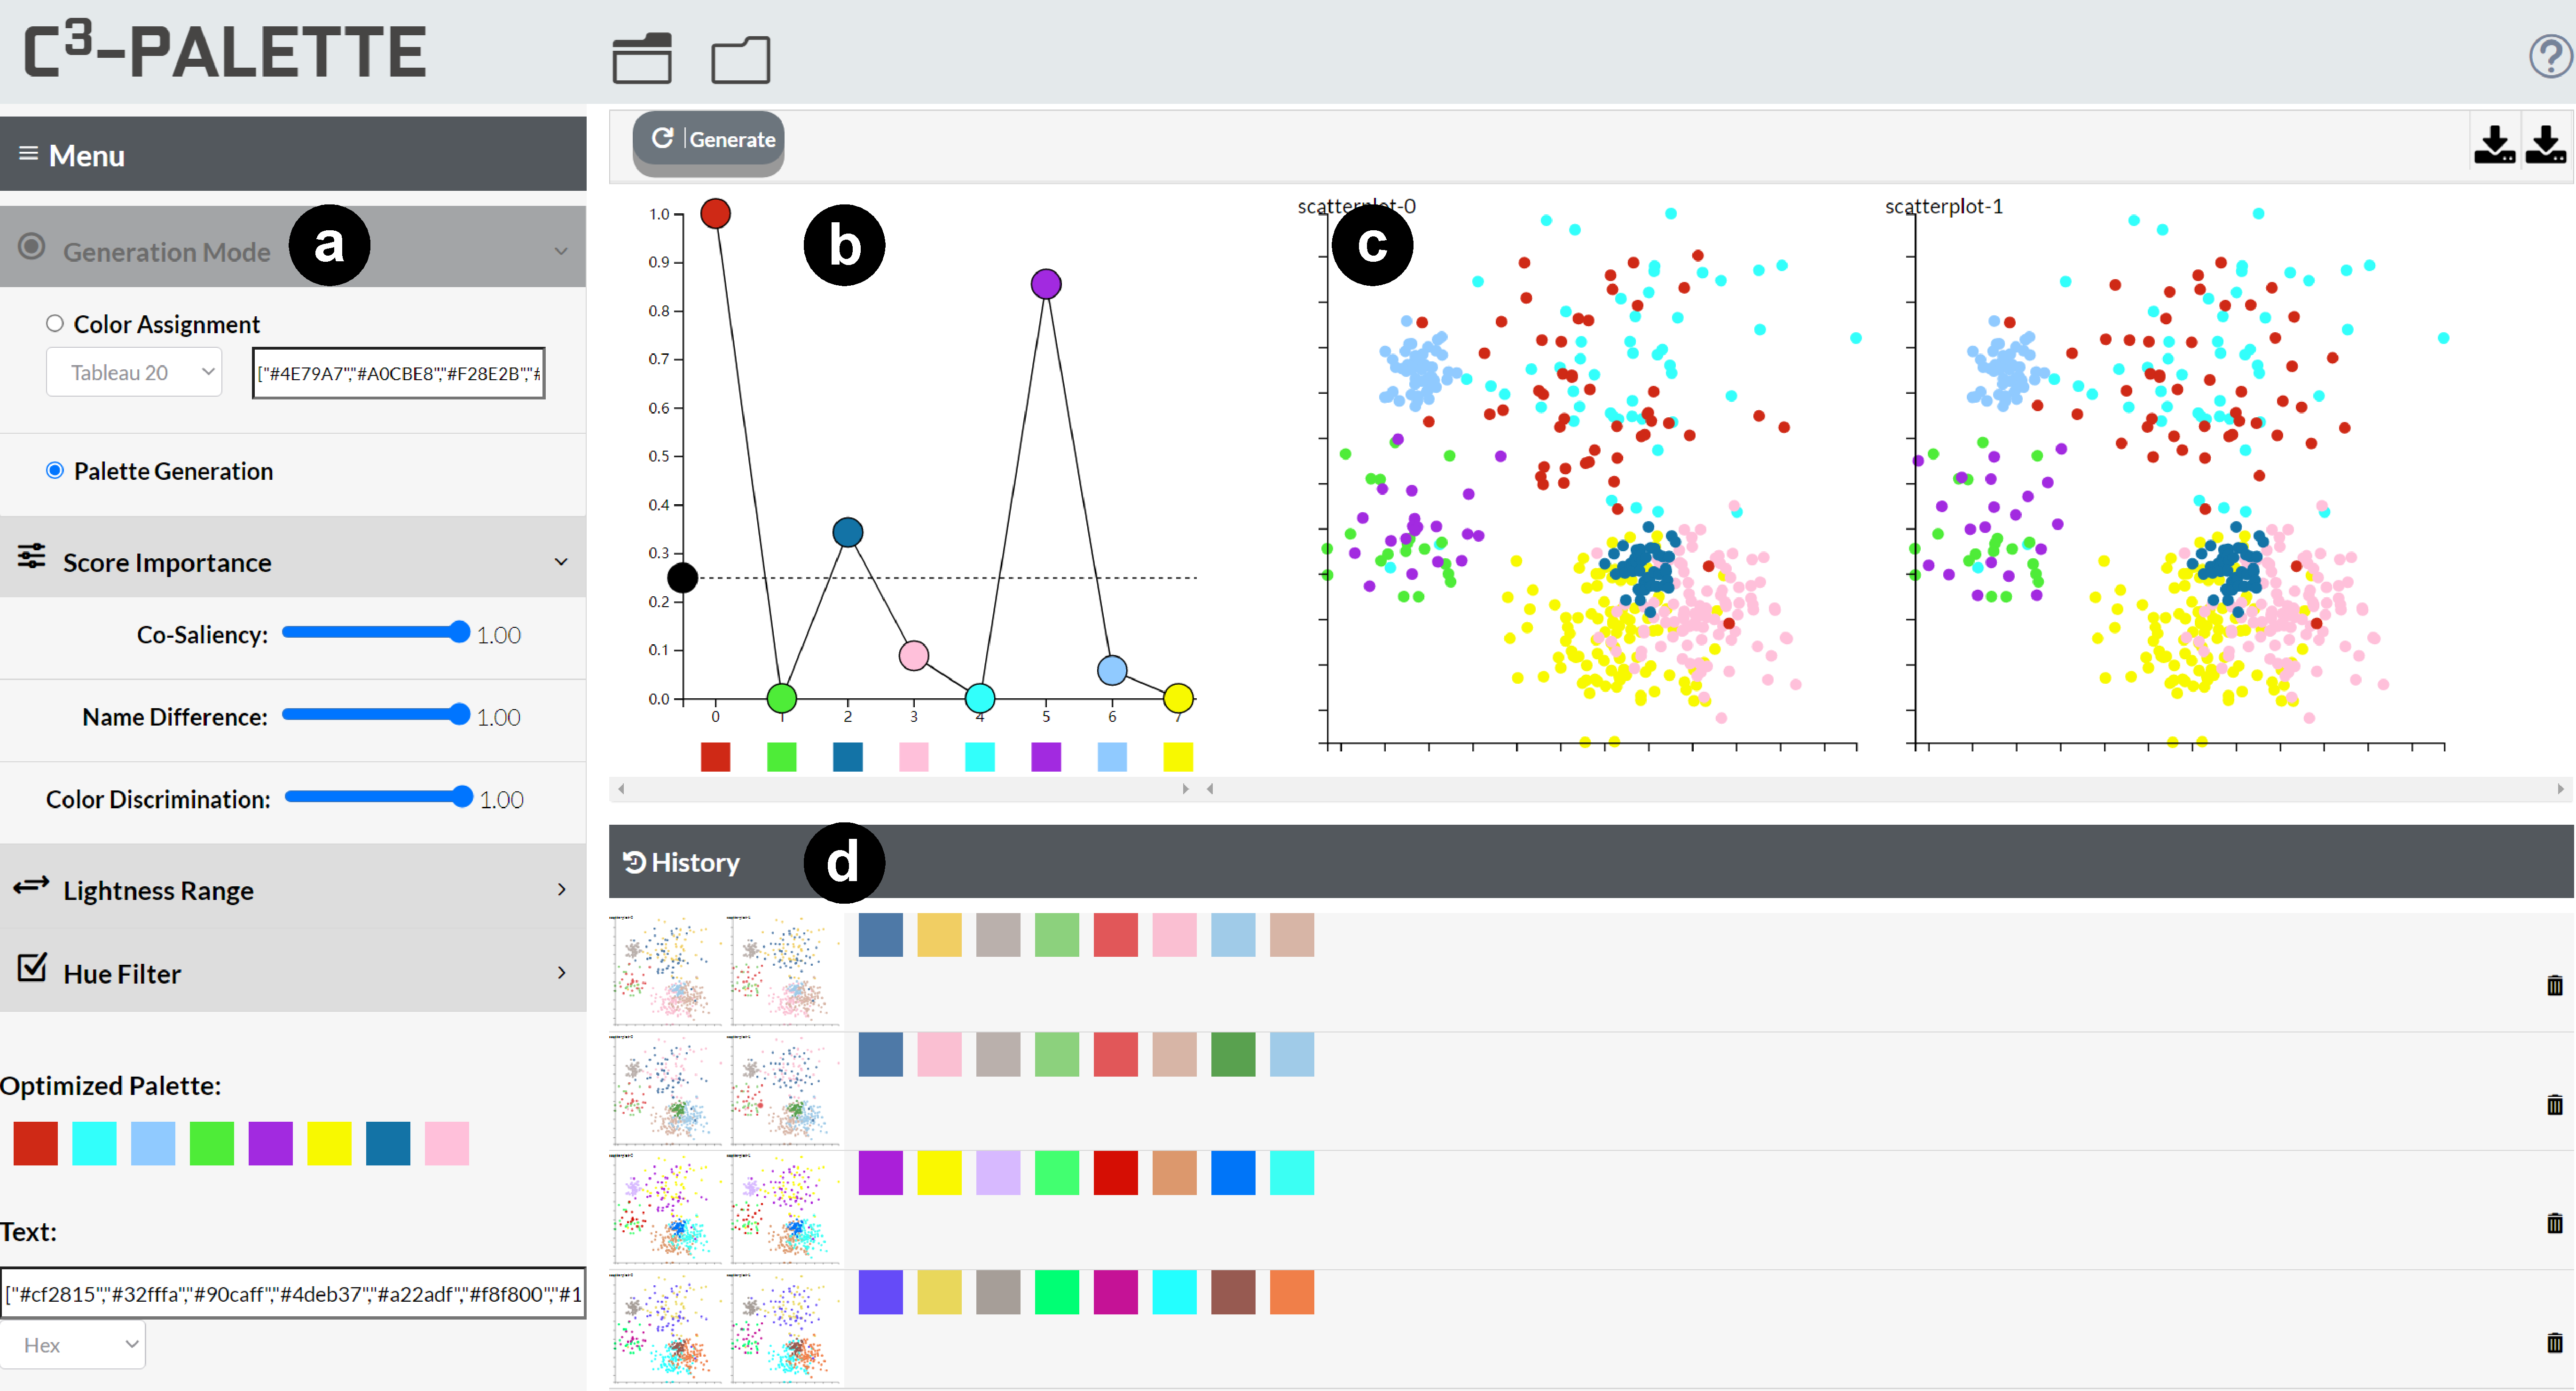
\includegraphics[width=0.8\columnwidth]{figures/interface.pdf}
\caption{Screenshot of the interactive system. (a) Settings Panel; (b) Control Panel; (c) Visualization Panel; (d) History Panel.}
\vspace*{-3mm}
\label{fig:ui}
\end{figure}

\section{Interactive System}
\label{sec:interaction}
To help users interactively design colors for comparing multi-class scatterplots, we developed a web-based multi-view visualization tool \footnote{\small \url{https://c3-palette.github.io/}} (see Fig.~\ref{fig:ui}).
It consists of four coordinated views: (a) a settings panel, (b) a control panel for adjusting importance threshold $\kappa$ and even importance value of each class, (c) the juxtaposed visualizations, and (d) a history view. The control panel shows the decision which classes are highlighted, and the history view allows to quickly explore and access previous color mappings.

After uploading multiple categorical scatterplots, the user can either choose a default color palette or use our system to automatically generate color palettes. In this case, the system automatically finds an optimal color mapping scheme to colorize the input data, while each class is encoded as a circle where the x-axis represents class label and the y-axis indicates the importance of each class. By default, the importance is represented by the change degree and $\kappa$ is set to zero. User can drag the circle to modify the corresponding importance value. The $\kappa$ is controlled by a black circle on the y-axis which can also be dragged to modify. Our system finds a color mapping scheme to highlight the classes with large importance and renders the classes in ascending order of the corresponding importance. If users like the color mapping scheme, they can save it to the history view.

\vspace{1.5mm}
\noindent\textbf{Flexible Importance Manipulation}.
Using $\theta_i$  defined in Eq.~\ref{eq:cosaliency}, the classes whose importance values are larger than the threshold $\kappa$ will be highlighted.
Fig.~\ref{fig:ui}(b,c) show an example, where the three classes with the adjusted importance values larger than $\kappa$ are emphasized with salient \emph{red}, \emph{blue} and \emph{purple} colors, respectively.
This control panel allows users to select arbitrary classes of interest to highhlight by simply adjust circle position and $\kappa$ value. More use cases can be seen in Sec.~\ref{sec:caseStudy}.

\vspace{1.5mm}
\noindent\textbf{Color Vision Deficiency}.
To help people with a color vision deficiency, we allow users to generate palettes that can be used for different types of vision problem, such as protanomaly and deuteranomaly which result in poor red-green hue discrimination. This is achieved by adopting a color blindness simulator(the source code can be find at github: https://github.com/MaPePeR/jsColorblindSimulator) and then used our matrix for palette evaluation. Fig.~\ref{fig:blindness} show an example, where the left two images show the auto-generated results and the right are the simulated results perceived by people with protanomaly.

\begin{figure}[ht]
\centering
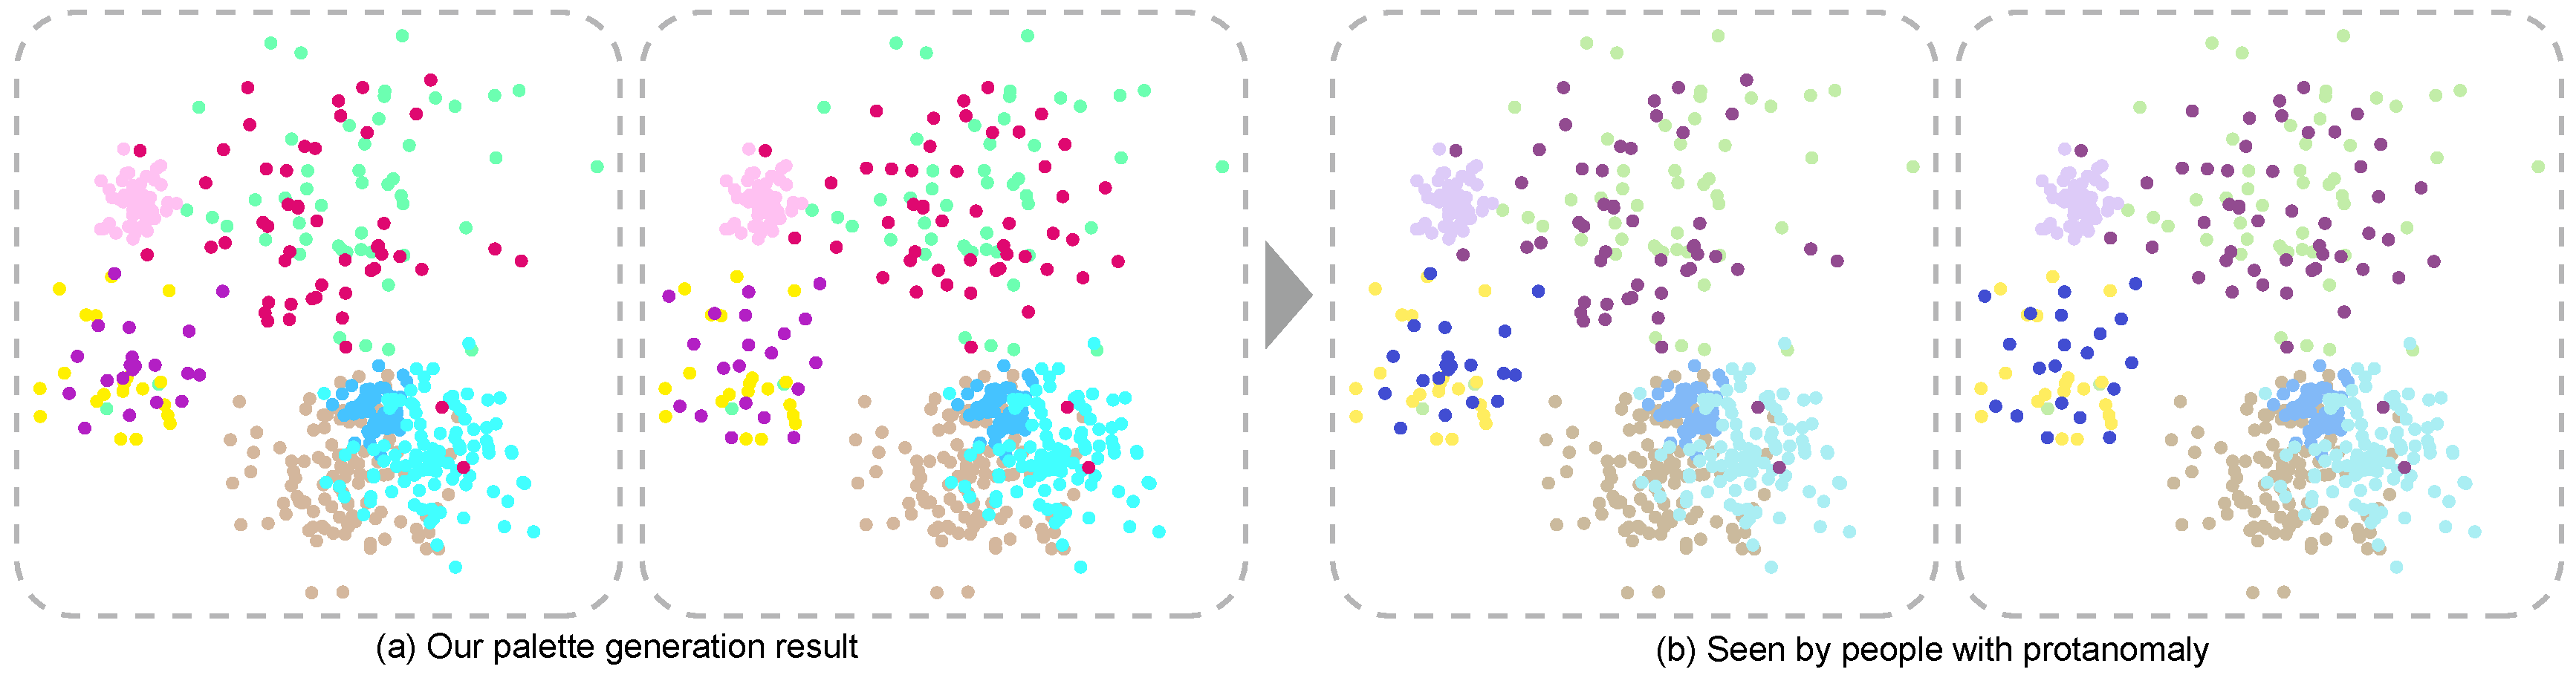
\includegraphics[width=0.96\linewidth]{figures/blindness.pdf}
\caption{Exploring the ability of our system to generate palettes for both people with normal vision and color blindness. (a) The automatic generated palette makes the two importance classes with large saliency while maintain good separability between other classes. (b) Simulated results for people with protanomaly. We can see our results maintain a good performance for color vision deficiency.}
\vspace*{-3mm}
\label{fig:blindness}
\end{figure}

